
%% trying not to mention ``h-value'' or ``g-value'' until it is defined

% \begin{abstract}
% Recent enhancements to greedy best-first search (GBFS) such as  DBFS, $\epsilon$-GBFS, Type-GBFS improve performance by occasionally
% introducing exploratory behavior which occasionally expands non-greedy nodes.
% However, most of these exploratory mechanisms do not address exploration within the space sharing the same heuristic estimate (plateau).
% In this paper, we show these two modes of exploration, which work across (\emph{inter-}) and within (\emph{intra-}) plateau, are complementary, and can be combined to yield superior performance. 
% % 
% We then introduces a new fractal-inspired scheme called Invasion-Percolation diversification,
% % We also introduce IP-diversification, a method combining Minimum Spanning Tree and randomization,
% which addresses  ``breadth''-bias instead of the ``depth''-bias addressed by the existing diversification methods.
% We evaluate IP-diversification for  both intra- and inter-plateau exploration,  and show that it  significantly improves  performance  in several domains.
% % 
% Finally, we show that combining diversification methods results in a planner which is competitive to the state-of-the-art for satisficing planning.
% \end{abstract}

\chapter{Analysis of Diversification Strategies for Greedy Best First Search}

Many search problems in AI are too difficult to solve optimally, and finding even one satisficing solution is challenging. 
Greedy Best-First Search (GBFS) is a best-first search variant where $f(n)$, the expansion priority of node $n$ is based only on a heuristic estimate of the node, i.e., $f(n) = h(n)$  (in contrast with \astar search, where the node priority also considers $g(n)$, the cost from the start state to $n$, and $f(n) = g(n)+h(h)$).
GBFS has been shown to be quite useful when it is necessary to find some  satisficing solution quickly, and GBFS 
has been the basis for \lsota domain-independent planners. % \cite{domshlak2015red}. % let's intentionally leave this ambiguous and not explicitly cite current sota planners, since we don't want our claims of ``improving upon sota'', ``competitive w. sota'' to be misunderstood as, e.g., ``better than gbfs/redblack''

Despite the ubiquitous use of GBFS for satisficing search,
previous work has shown  that GBFS is susceptible to being 
easily trapped by undetected dead ends and huge search plateaus.
On infinite graphs, GBFS is not even complete \cite{Valenzano2016}
because it could be misdirected by the heuristic guidance forever.
These pathological behaviors are caused by the fact that 
the search behavior of GBFS strongly depends on the
quality of the heuristic function.

%Existing methods tackle this issue from two directions.
Previous approaches to this problem can be classified into two classes.
The first class of methods focuses on an issue arising with inadmissible heuristics,
which can incorrectly label nodes which are close to the goal (low $h^*$, optimal cost to goal) as unpromising (overestimation: $h>h^*$), 
causing GBFS to delay expanding them until all other open nodes with smaller $h$-values have been expanded.
Several approaches have been proposed for alleviating this problem, including 
DBFS \cite{imai2011novel}, $\epsilon$-GBFS \cite{valenzano2014comparison} and Type-GBFS \cite{xie14type}.
These approaches \emph{diversify} the search by occasionally expand nodes which do not have the lowest $h$-value, 
and provide an opportunity to expand nodes that are mistakenly overlooked due to  heuristic errors.

The second class of methods focuses on a different issue which arises in both admissible and inadmissible heuristics:
A node that is far from the goal (high $h^*$) can be mislabeled as promising (underestimation: $h<h^*$), 
causing GBFS to have larger plateaus and expand unnecessary nodes.
Techniques which address this issue include  \emph{plateau escaping} \cite{Coles07}, \emph{local exploration} \cite{XieH14gbfsle} or \emph{tiebreaking} \cite{Asai2016}.

%% this paragraph is important because diversity, exploration, and
%% ``removing bias'' might not immediately connect with each other
All of these methods share the objective of removing some \emph{bias},
thereby encouraging  \emph{exploration} by the search process
and adding \emph{diversity} in decision making process.
In this paper, we use the terms ``exploration'', ``diversity'', and ``bias removal'' interchangeably.
Previous work lacked a common framework which unified these various approaches to diversification/exploration/bias removal.
Furthermore, as shown later, the current \lsota methods are based on diversification with respect to search depth (distance from the start / goal / plateau entrance),
so the bias among the set of nodes with the same search depth is not removed.

In this paper, we first show that  the above two classes of approaches to diversification are orthogonal and should be combined for better performance.
We show that a recently proposed depth-based tie-breaking strategy for \astar \cite{Asai2016} also improves the performance of GBFS by diversifying the depth within each h-plateau.
Both depth diversification strategy and Type-GBFS are shown to be instances of a \emph{type}-based diversification strategy \cite{xie14type}: Depth diversification applies type-based diversification within a plateau, and Type-GBFS applies it between plateaus.
We compare their empirical performance and show that their improvements are complementary -- 
They improve the performance in different domains, and a configuration using both methods, achieves the best overall coverage.
This effectively shows that \emph{inter}-plateau and \emph{intra}-plateau diversification are two orthogonal usages of diversification, and both modes should be used if possible.
 
Next, we propose and evaluate a new diversification strategy called IP-diversification which addresses diversity with respect to \emph{breadth}.
We evaluate this new diversification strategy both for intra-plateau and inter-plateau exploration.
Complementary effects on intra/inter-plateau exploration were similarly observed. In addition, IP-diversification outperforms the Type-based diversification strategy.
Finally, we show that by combining several intra/inter plateau exploration strategies, we can improve upon \lsota planners in terms of coverage.
% The FD implementation of "Type-LAMA" is not the same as the Jasper code which competed in IPC2014, so can't say anything aobut Type-LAMA IPC performance rank.
%(LAMA, the IPC2011 winner,  and Type-LAMA, the non-portfolio planner with the highest coverage in IPC2014) in terms of coverage.

\section{Preliminaries and Background}

We first define some notation and the terminology used throughout the
rest of the paper.
$h(n)$ denotes the estimate of the cost from the current node $n$ to the nearest goal node.
$g(n)$ is the current shortest path cost from the initial node to the current node.
$f(n)=g(n)+h(n)$ is the estimate of the resulting cost of the path to a goal
containing the current node.
We omit the argument $(n)$ unless necessary.
$h^*,g^*$ and $f^*$ denotes the true optimal cost from $n$ to
a goal, from the start to $n$, or from the start to a goal through $n$, respectively.

A \emph{sorting strategy} for a best first search algorithm 
tries to select a single node from the open list (OPEN).
Each sorting strategy is denoted as a vector of several \emph{sorting criteria}, such as
[$\text{criterion}_1$, $\text{criterion}_2$, $\ldots$,
$\text{criterion}_k$], which means: First, select a
set of nodes from OPEN using $\text{criterion}_1$.  If there are still multiple
nodes remaining in the set, then break ties using $\text{criterion}_2$
and so on, until a single node is selected.  The \emph{first-level
sorting criterion} of a strategy is $\text{criterion}_1$, the
\emph{second-level sorting criterion} is $\text{criterion}_2$, and so on.

Using this notation, \astar without any tie-breaking can be
denoted as $[f]$, and \astar which breaks ties according to $h$
value is denoted as $[f,h]$. Similarly, GBFS is denoted as 
$[h]$.  Unless stated otherwise, we assume the nodes are sorted in
increasing order of the key value, and BFS always selects a node with the smallest
key value.

A sorting strategy fails to select a single node when some nodes
share the same sorting keys. In such cases, a search algorithm must
select a node according to a \emph{default} tie-breaking
criterion, $\text{criterion}_k$, such as \fifo (first-in-first-out), \lifo
(last-in-first-out) or \ro (random ordering).
For example, an \astar using $h$ and \fifo tie-breaking is denoted as $[f,h,\fifo]$.
By definition, default criteria are guaranteed to return a single node from a set of
nodes. When the default criterion does not matter, we may use a wildcard $*$ as in $[f,h,*]$.

Given a search algorithm with a sorting strategy, 
a $\plateau{\text{criterion}\ldots}$ is a set of nodes in OPEN which share
the same sort keys according to non-default sorting criteria and therefore
are indistinguishable. In a case of \astar
using tie-breaking with $h$ (sorting strategy $[f,h,*]$), the plateaus are denoted as
$\plateau{f,h}$, the set of nodes with the same $f$ cost and the same $h$ cost.
We can also refer to a specific plateau with $f=f_p$ and $h=h_p$ by $\plateau{f_p,h_p}$.

Finally, OPEN list \emph{alternation}  \cite{RogerH10} is a technique to combine multiple
sorting strategies in order to improve the robustness of the search algorithm.
Nodes are simultaneously stored and sorted into
independent OPEN lists with different strategies, and
node expansion alternates among the OPEN lists.
We denote an alternating OPEN list as $\mit{alt}(X_1,X_2,\ldots)$ where
each $X_i$ is a sorting strategy.

\subsubsection{Depth-Based Tie-breaking}

To date, there has been relatively little work on 
tie-breaking policies for BFS.

Recently, \citeauthor{Asai2016} (\citeyear{Asai2016}) performed an in-depth investigation
of tie-breaking strategies for \astar, in which
the tie-breaking policy was found to have a
significant effect on the performance when the search plateau is huge.
In the most commonly used  sorting strategies, $[f,h,\fifo]$ or $[f,h,\lifo]$, the search has a strong bias to focus on  either the regions of smaller (\fifo) or larger (\lifo) search depth of each $\plateau{f,h}$, which can cause a failure to find a solution within a given time limit.

To address the issue caused by the search bias within a plateau,
they proposed a notion of \emph{depth} and diversified the search over different depths
within a plateau. The depth $d(n)$ of a state $n$ is an integer representing 
the step-wise distance from the \emph{entrance} of the plateau (the most recent state which
entered the plateau, along the path from the initial state). 
% 
$d(n)=d(m)+1$ when $n$ and the parent node $m$ are on the same plateau.
For example, with strategy $[f,h,*]$, 
$\plateau{f(n),h(n)}=\plateau{f(m),h(m)}$, therefore
$f(n) = f(m) \land h(n) = h(m)$.
$d(n)$ is 0 otherwise.
The nodes are stored in buckets indexed by depth, and expansions are allocated across different buckets with equal probability at every iteration.
The resulting sorting strategy is denoted as $[f,h,\depth,*]$.

For GBFS, to our knowledge, there is currently no
well-established tie-breaking policy analogous to $h$-based tie-breaking for \astar.
Presumably, this is  because
while \astar has access to three cost values ($f$, $g$, and $h$),
%% better to keep this footnote even without citations, just so we acknowledge that there are some "obvious" tiebreaking strategies.
GBFS is guided solely by the heuristic value $h$.\footnote{Tie-breaking based on  $g$ is sometimes used, but this is motivated as a means to find higher-quality solutions. To our knowledge, in a satisficing context, tie-breaking strategies for reducing search effort have not been explicitly motivated or evaluated.} 
As a consequence,
improvements to  GBFS have been primarily achieved by addressing other aspects, such as
modifying the evaluation scheme \cite[lazy evaluation]{richter2010lama}, queue alternation
(multiple heuristic functions), preferred operators \cite{hoffmann01}, and diversification.

\subsubsection{Exploration Mechanisms}

One class of improvements to GBFS seeks to introduce exploration (diversity) to the search process, as exemplified by DBFS \cite{imai2011novel}, $\epsilon$-GBFS \cite{valenzano2014comparison}, Type-GBFS
\cite{xie14type}.
These algorithms address the problem of GBFS getting stuck due to heuristic errors.
GBFS will not expande a node $n$  until it expands all nodes with a lower $h$-value than $n$.
Thus, search progress can be delayed when a good (low-$h^*$) node is mistakenly assigned a poor (high) $h$-value (overestimation), or bad (high-$h^*$) nodes are assigned promising $h$-values (low-$h$, underestimation).
These exploration strategies allow the search to escape local minima by relaxing the $h$-based best-first node expansion order.

KBFS(k) \cite{felner2003kbfs} attempts to address this problem by expanding $k$ nodes at a time.
% in order to prevent the search algorithm from getting stuck in a heuristic trap.
%  KBFS provided an
% interesting observation to GBFS --- KBFS(1) is equivalent to GBFS, and
% KBFS($\infty$) is equivalent to Breadth-First Search.
% 
% 
$\epsilon$-GBFS \cite{valenzano2014comparison} selects a random node from OPEN with some fixed probability $\epsilon <1$.
This is a randomized, weighted alternating 
OPEN list using $[h,*]$ and $[\ro]$ (no sorting criteria): $\mit{alt}([h,*],[\ro])$.

While $\epsilon$-GBFS relies on  a pure randomization strategy to escape traps and introduce exploration, 
Type-GBFS \cite{xie14type} explicitly seeks to remove bias and diversify the search  by categorizing OPEN according to several key values, such as $[g,h]$ for each state.
Each node is assigned to a bucket according to its key value.
The search then selects a random node in a random
bucket, avoiding the cardinality bias among buckets.
Since Type-GBFS does not sort the buckets according to the key vector, we use a different notation $\brackets{\ldots}$,
such as $\brackets{g,h}$ denoting type buckets whose key values are $g$ and $h$.
In the implementation evaluated by \citeauthor{xie14type} (\citeyear{xie14type}),
Type-GBFS alternates the exploitative (standard best-first order) expansion and the exploratory (randomized) expansion. We denote this 
 as $\mit{alt}([h,*], [\brackets{g,h},\ro])$.

DBFS \cite{imai2011novel} diversifies the
search based on $g$ and $h$ values, but with several key differences from
the above two algorithms: First, the exploratory selection is not uniformly
random, but is subject to a particular distribution function based on 
$h, g, h_{min}$ and $g_{max}$. Second, it uses a local search with
a bounded number of expansions equal to $h$, which dynamically balances the exploration
and exploitation --- it does more GBFS when $h$ is large (far
from the goal), and less GBFS near the goal ($h$ is small).

GBFS with Local Exploration (GBFS-LE) introduces a 2-level search architecture which runs
GBFS until it detects that no improvements have been made for a while, and
then runs a local GBFS (GBFS-LS) or random walk (GBFS-LRW)
in order to find an exit to a more promising region of the search space \cite{XieH14gbfsle}.

\section{Intra- and Inter-plateau Diversification}
\label{sec:intra-inter}

Previous works on exploration for GBFS  address the problem of heuristic errors
by occasionally expanding nodes with high $h$.
Since this type of diversification operates  across different search plateaus,
we refer to these as \emph{inter-plateau} exploration.
However, we propose another type of exploration,
which we call \emph{intra-plateau} exploration, which works within a particular plateau.
This type of exploration only changes expansion order among the nodes within a plateau.
We use this new term rather than tiebreaking in order to emphasize its relationship to plateaus.

Existing inter-plateau exploration can be understood as a diversification applied to $h^*$ plateau.
Consider a hypothetical  2-dimensional histogram (\refig{fig:h-hstar}) of the number of nodes for each pair $h,h^*$.
If both axes were $h^*$ (i.e., $h$ is a perfect heuristic), all nodes would be on the diagonal line $x=y$.
However, in reality, $h$ has errors relative to  $h^*$, as would be shown if we projected the histogram to the $x$-axis.
Since low-$h^*$ nodes may have high-$h$ values,
it is sometimes reasonable to expand
high-$h$ nodes depending on the distribution defined by the problem characteristics and the heuristic function.
% To our knowledge, all previous work on exploration for GBFS has addressed exploration along this dimension by ignoring the best-first ordering wrto $h$.

\begin{figure}[bt]
 \centering
 \includegraphics{img/h-hstar.pdf}
 \caption{A conceptual view of the node distribution wrto $h^*$ and inadmissible $h$.
 The peak line on the surface is on $x=y$.
 Projection to $x$-axis shows the distribution of $h$ values, while 
 projection to $y$-axis shows the distribution of $h^*$ values.
 }
 \label{fig:h-hstar}
\end{figure}

However, the converse can also be true --
not only can a single $h^*$-plateau consists of nodes with different $h$ values,
a single $h$-plateau consists of nodes with different $h^*$ values,
as would be shown by projecting the histogram  to the $y$-axis in \refig{fig:h-hstar}.
This leads to an observation that
\emph{in the worst case, a naive algorithm may keep expanding bad (high-$h^*$) nodes within an $h$-value plateau}.

More precisely, the node selection algorithm of a diversified GBFS variant can be described as follows:
\begin{defi}
 An \emph{inter}-plateau diversification strategy for GBFS is a method for selecting the next $h$-value.
\end{defi}
\begin{defi}
 An \emph{intra}-plateau diversification strategy for GBFS is a method for selecting the next node in the plateau selected by an \emph{inter}-plateau strategy.
\end{defi}
This view cleanly separates the effects of two strategies, providing a firm basis for the observation that their effects are orthogonal and should be combined for the better performance.
It is straightforward to see that,
given an OPEN list state and an inter-plateau diversification strategy,
the next h-plateau to select a node from is independent of intra-plateau strategy.
Likewise, given a set of nodes with the same $h$-value and an intra-plateau (tiebreaking) strategy,
the next expanded node is independent of inter-plateau strategy.

Intra-plateau diversification is similar to \emph{local exploration} \cite{XieH14gbfsle,XieMH15}, but is more restrictive. \emph{Local exploration} is targeted for uninformative heuristic region (UHR), which includes both plateaus and local minima. In fact, GBFS-LS does not restrict the local exploration by the $h$-value, thus it may eventually expand a different plateau as the side effect.
Similarly, some existing inter-plateau strategies such as $\varepsilon$-greedy GBFS have some intra-plateau side-effects because they may distort the expansion order within a plateau.

%% this explanation is ambiguous, so I left it out.
% \emph{Unlike inter-plateau exploration, which addresses \textbf{incorrect information for h$^*$-plateau},
% intra-plateau exploration addresses the problem of \textbf{insufficient information for h-plateau.}}
% %An intra-plateau diversification tries to expand low-$h^*$ nodes within an $h$-value plateau
% %with a sufficient probability.
% %% ``trap'' may refer to specific structure defined in ``Traps, invariant and dead-ends'' lipo/muise
% 
%% below is just repeating the previous statements, so left out in favor of space.
% An intra-plateau exploration strategy tries to avoid the aforementioned pathology of continually expanding high-$h^*$ nodes within an $h$-value plateau.
% Since we do not know \emph{a priori} which nodes in an $h$-plateau are better (low-$h^*$) than the other nodes in the same $h$-plateau, by
% an  adversary argument, the safest strategy is to avoid biased choices  -- 
% in the absences of useful heuristic knowledge which differentiates among a set of nodes, 
% an expansion policy which is biased to expand some particular group of states within a plateau can be exploited by an adversary which seeks to hide better (low-$h^*$) nodes.

\subsubsection{Type-Based Diversification}

The notions of inter-vs-intra plateau exploration allows us to discuss and compare depth diversification \cite{Asai2016} and Type-GBFS \cite{xie14type} within a unified framework
 -- it turns out that
these are essentially the same basic idea,  applied to different contexts (inter-vs-intra plateau, satisficing-vs-optimal search), using different parameters (type systems).

\citeauthor{lelis2013stratified} (\citeyear{lelis2013stratified}) define a general framework for adding exploration to search using ``type systems'':

%% for future reference, to see how much our definition drifts from the original
%\begin{defi} %Definition, copied from Xie's TypeGBFS paper (2014). This is almost the same as the original def in Lelis et al 2013, except the original def was for a search tree.
%  Let $S$ be the set of nodes in the search space. $T = \{t_1,...,t_n \}$ is a type system for $S$  if $T$ is a disjoint partitioning of $S$. For every $s \in S$, $T(s)$ denotes the unique $t \in T$ with $s \in S$.
%\end{defi}
%They define a type bucket $tb$ which partitions nodes according to their type, and they define type bucket-based node selection as: pick a bucket $b$ uniformly at random from all non-empty buckets. Then, pick a node uniformly at random from $b$.
%Type-GBFS alternatively expands a node from the regular open list $O$ and from this type bucket, where new nodes are added to both $O$ and $tb$.

\begin{defi} 
A \emph{Type system} \cite{lelis2013stratified} is a 
function from a node to a vector,
$T: \text{node} \rightarrow \mathbb{Z}^k, T(n)=\brackets{t_1(n) \ldots t_k(n)} $, where each function $t_i(n)$ returns an integer for each node $n$.
\end{defi}

%% These functions are assumed to represent the characteristic feature of the state.

\citeauthor{xie14type} proposed a node selection technique based on type systems.

\begin{defi}
% \emph{Type-Based Diversification} 
 \emph{Type-Based Node Selection} \cite{xie14type}
with a type system $T(\cdot)$ of $k$ types maintains a $k$-dimensional matrix of sets of nodes,
 where each set $S_v$ is associated with a vector $v=\brackets{v_1,\ldots,v_k}$.
 Each node $n$ is stored in $S_{T(n)}$.
 For dequeueing, it randomly selects a non-empty set from all sets,
 and a random node in the set is dequeued.
\end{defi}

The reason for selecting a set at random is to try to allocate the search effort among a diverse set of nodes.
Some sets could contain a large number of nodes while others are only scarcely populated.
Type-based node selection tries to remove this cardinality bias among buckets.
Because type-based node selection  has this diversification as an explicit goal and is best understood as a diversification strategy, we call it \textbf{\emph{type-based diversification}} in the rest of this paper.

% describe Type-GBFS first to keep the description of all the type-based previous work together.
Type-GBFS \cite{xie14type} uses type-based diversification with type system $\brackets{g,h}$ for inter-plateau
exploration. Their inter-plateau exploration is implemented by queue alternation \cite{RogerH10} between
standard Best-First queue and type-based diversification queue.

Depth diversification \cite{Asai2016} originally addressed the issue of zero-cost actions in admissible search with \astar,
and the configuration was denoted as $[f,h,\depth]$ using the type system notation, where $f=g+h$ and $d$ is a number of steps from the current node to the nearest ancestor that has the different $h$-value.
In order to use $\depth$ for GBFS, the resulting configuration is $[h,\depth]$.
This configuration is considered an instance of intra-plateau type-based diversification because
it uses type-based diversification $\depth$ for diversifying the search within plateaus defined by $h$.

%% removed Type-GBFS with <h>. Type-GBFS with <g,h> turns out to be just sufficient for discussion.

\subsection{Empirical Comparison of Intra- and Inter-Plateau Exploration}
\label{sec:gbfs-comparison}

 % changed to "complementary" in the rest of the section, "complementary" is used to talk about coverage performance on domains, while "orthogonal" refers to the algorithmic behavior and what issues each addresses.

Since depth-diversification and Type-GBFS turned out to be instances of the same strategy applied for different purposes
(intra/inter-plateau), we use these as exemplars to compare the impact of intra/inter-plateau exploration.
In the following experiments, we empirically show that they achieve complementary performance improvements.
This indicates that inter/intra-plateau exploration in fact addresses orthogonal issues of \emph{incorrect} and \emph{insufficient} information, respectively.
We then show that intra/inter-plateau exploration can be successfully combined in a single search algorithm.

We compare the performance of the following configurations for Greedy best-first search using the Fast Forward heuristic $\ff$ \cite{hoffmann01} and Causal Graph heuristic $\cg$ \cite{Helmert04}.
\begin{itemize}
\item \bi{h}: baseline GBFS (eager evaluation).
\item \bi{hd}: Depth diversification \cite{Asai2016} -- intra-plateau type-based diversification, $[h,\depth]$.
\item \bi{hD}: Type-GBFS \cite{xie14type} -- inter-plateau type-based diversification,  $alt([h],[\brackets{g,h},\ro])$,
\item  \bi{hdD}: A combined configuration of intra- and inter-plateau type-based diversification, $alt([h,\brackets{d}],[\brackets{g,h},\ro])$.
\end{itemize}

Experiments are conducted on a Xeon E5-2666 @ 2.9GHz, HyperThreading and TurboBoost disabled.
We used IPC 2011 and 2014 instances with a 4GB memory limit and 5 minutes time limit. Since IPC 2011 and IPC 2014 contain duplicate domains, we removed duplicates from the 2011 set, keeping the 2014 versions.
All implementations are based on FastDownward \cite{Helmert2006} and
unless specified, all configurations use \fifo default tiebreaking (FastDownward default).
% 
Following previous work \cite{valenzano2014comparison,xie14type}, all configurations are evaluated under unit cost transformation
because we focused on the coverage (number of problems solved within resource limit) for purely satisficing search. 
Each experiment is run 10 times, and the means are shown in \reftbl{tbl:results}.

First, 
% 
intra-plateau exploration \bi{hd} increases coverage for both heuristics
$\cg$ ($187 \rightarrow 194.2$) and $\ff$ ($192 \rightarrow 223.9$).
This shows that intra-plateau exploration successfully allows GBFS to avoid being trapped in $h$-value plateaus.
Inter-plateau exploration \bi{hD} also increases coverage for both heuristics, confirming the results in \cite{xie14type}.
It is worth mentioning that the performance of \bi{hd} is comparable to \bi{hD}, showing that intra-plateau exploration is no less important than inter-plateau exploration which previous work focused on.

Second, the data shows that the effects of inter/intra-plateau exploration are complementary, 
as would be expected since they are designed to address orthogonal issues.
In most cases,
when \textbf{hd} improves upon \textbf{h} then \textbf{hdD} improves upon \textbf{hD},
and when \textbf{hD} improves upon \textbf{h} then \textbf{hdD} improves upon \textbf{hd}.
As a result, for both $\cg$ and $\ff$ heuristics, the \textbf{hdD} configuration had higher coverage ($\cg$:215.8, $\ff$:223.9) than the hd ($\cg$:194.2, $\ff$:208) and hD ($\cg$:206.1, $\ff$:207.4) configurations. 
This shows that combining intra/inter-plateau exploration methods which address orthogonal issues results in better overall performance than either type of exploration by themselves.
% in the earlier version, we said this in the IP evaluation section, but better to highlight this result in this section so it's obvious the result is independent of IP and increase the value of the novel inter/intra framework.

% \section{parallel "quicksummary -f 1,4,7 finished/gbfs-\{1\}-fifo/*/*\{2\}*" ::: cg ff ::: 2011 2014}
\label{sec-1}

\section{}
\label{sec-2}

\section{format}
\label{sec-3}


\begin{table}[htb]
 \setlength{\tabcolsep}{0.3em}
\centering
\relsize{-1}
% \begin{tabular}{|ll|r|rrr||r|rrr|}
\begin{tabularx}{\linewidth}{|rl|XXXX||XXXX|}
\hline
& & \multicolumn{ 4}{c||}{$\cg$} & \multicolumn{ 4}{c|}{$\ff$} \\ 
& & h & {hd}    & {hD}    & {hdD}  & h & {hd}    & {hD}    & {hdD}  \\ 
& &   & {intra} & {inter} & {both} &   & {intra} & {inter} & {both} \\ 
\hline
   % &total       & 228 & 241.1        & 245.1          & \textbf{263.2} & 231 & 264.3         & 252.9          & \textbf{280.6} \\ \hline \multirow{14}{0.3em}{\rotatebox{90}{\textbf{IPC2011}}}
   &total       & 187 & 194.2        & 206.1          & \textbf{215.8} & 192 & 208           & 207.4          & \textbf{223.9} \\ \hline \multirow{8}{0.3em}{\rotatebox{90}{\textbf{IPC11 w/o duplicates}}}
 % &barman      & 0   & 0            & 0              & 0              & 8   & \borange{8.6} & \borange{10.9} & \borange{10.3} \\ 
   &elevators   & 9   & 8            & 8.7            & \textbf{9.7}            & 19  & 14            & 15.9           & 13.7           \\ 
 % &floortile   & 0   & 0            & \bred{2.1}     & \bred{2}       & 6   & 6.1           & \bred{7.1}     & \bred{6.9}     \\ 
   &nomystery   & 7   & 6            & \bred{15.4}    & \bred{15.1}    & 9   & 7             & \bred{16.6}    & \bred{17}      \\ 
 % &openstacks  & 10  & \bblue{14.7} & 9.9            & \bblue{12.8}   & 11  & \bblue{18.6}  & 11             & \bblue{15.8}   \\ 
   &parcprinter & 20  & 20           & 19.4           & 18.7           & 20  & 20            & 20             & 20             \\ 
 % &parking     & 18  & 17.7         & 11.6           & 14.1           & 11  & \bblue{20}    & 10.4           & \bblue{17.2}   \\ 
   &pegsol      & 20  & 20           & 20             & 20             & 20  & 20            & 20             & 20             \\ 
   &scanalyzer  & 20  & 20           & 19.9           & 20             & 15  & 15.1          & \bred{18}      & \bred{18.6}    \\ 
   &sokoban     & 16  & 16           & \bred{16.9}    & \bred{17}      & 19  & 19            & 17.4           & 17.4           \\ 
   &tidybot     & 16  & \borange{18} & \borange{18.7} & \borange{18.6} & 16  & 16            & 16             & \textbf{16.7}  \\
 % &transport   & 10  & \bblue{11.5} & 9              & \bblue{12.1}   & 0   & 0             & 0              & 0.2            \\ 
 % &visitall    & 3   & 3            & \bred{6.4}     & \bred{6.4}     & 3   & 3             & \bred{6.1}     & \bred{6.3}     \\ 
   &woodwork    & 2   & 2            & \bred{2.7}     & \bred{7.7}     & 2   & 2             & \bred{4}       & \bred{7.2}     \\ \hline \multirow{14}{0.3em}{\rotatebox{90}{\textbf{IPC14}}}
   &barman      & 0   & 0            & 0              & 0              & 0   & 0             & \bred{1.5}     & \bred{1}       \\ 
   &cavediving  & 7   & 7            & 7              & 7              & 7   & 7             & 7              & 7.2            \\ 
   &childsnack  & 1   & \bblue{6}    & 0.1            & \bblue{1.5}    & 0   & \bblue{4}    & 0              & \textcolor{blue}{0.3}            \\ 
   &citycar     & 0   & 0            & \bred{7.8}     & \bred{4.7}     & 0   & 0             & \bred{7.2}     & \bred{7.1}     \\ 
   &floortile   & 0   & 0            & \bred{2}       & \bred{2}       & 2   & 2             & 2              & 2.1            \\ 
   &ged         & 0   & 0            & \bred{9.6}     & \bred{9.7}     & 19  & 19            & 14             & 13.8           \\ 
   &hiking      & 18  & 16.9         & \bred{19.5}    & \bred{19.7}    & 20  & 20            & 19.8           & 20             \\ 
   &maintenance & 16  & 16           & 16.1           & 15.8           & 11  & 8             & 10.7           & 11.1           \\ 
   &openstacks  & 0   & \bblue{3.5}  & 0              & \bblue{0.5}    & 0   & \bblue{12.6}  & 0              & \bblue{7}      \\ 
   &parking     & 7   & \bblue{9.7} & 1.2            & \textcolor{blue}{4.1}            & 4   & \bblue{7.5}   & 1.4            & \bblue{5.7}    \\ 
   &tetris      & 18  & 17.1         & 12.4           & 14.3           & 1   & \bblue{5.8}   & 3.2            & \bblue{4.9}    \\ 
   &thoughtful  & 5   & 5            & 5              & 5              & 8   & \borange{9}   & \borange{12.7} & \borange{13.1} \\
   &transport   & 5   & 3            & 3.7            & 4.7            & 0   & 0             & 0              & 0              \\ 
   &visitall    & 0   & 0            & 0              & 0              & 0   & 0             & 0              & 0              \\ 
\hline
\end{tabularx}
% \end{tabular}
\caption{
Number of solved instances (5 min, 4GB RAM), mean of 10 runs.
\textbf{h}: baseline GBFS.
\textbf{hd/hD}: intra/inter-plateau type-based diversification $[h,\depth]$ and
  $alt([h],[\brackets{g,h},\ro])$ (Type-GBFS),
\textbf{hdD}: A combined configuration, $alt([h,\brackets{d}],[\brackets{g,h},\ro])$.
 % -- (\textbf{see supplements for \lifo and \ro}).
\textbf{Bold} indicates that (improvements vs. baseline)$>0.5$.
\textcolor{blue}{Blue} indicates that \textbf{hdD} improvement correlates with \textbf{hd} (intra-plateau) improvement,
\textcolor{red}{red} indicates that \textbf{hdD} improvement correlates with \textbf{hD} (inter-plateau) improvement,
and \textcolor{orange}{orange} indicate that both intra/inter-plateau schemes as well as the combined \textbf{hdD} scheme improved.
Thus, intra- vs. inter-plateau scheme have complementary effects 
that improve \textbf{hdD}.
}
\label{tbl:results}
\end{table}




Based on these results, we conclude that:
%% inline list from enumitem
% \begin{enumerate*}
\begin{enumerate} % there's space, and these are the strongest results in the paper, so let's enum
\item Inter- and intra-plateau exploration address orthogonal issues and have complementary performance; 
%While the depth diversity $[h,\depth]$ and Type-GBFS $\brackets{h}$ configurations are both instances of bucket-based diversification,  
%the way it is used has affected the performance.
% XXX since these configs use different keys, it seems safer to avoid emphasizing that they are "the same"
%% this second element is not so important
% \item The benefits from each type of diversification (inter/intra-plateau) depend on the problem domain and heuristic used; and
\item Combining inter- and intra-plateau exploration can result in better performance than either  exploration alone.
\end{enumerate}
% \end{enumerate*}

\section{Breadth-Based Diversification:\\ Invasion Percolation}
\label{sec:ip}
\subsubparagraph{intro}

A limitation of  type-based diversification based on path distance % path dist estimates are included in in ``based on path dist''
is that it does not diversify with respect to breadth -- 
nodes with equal estimated distance from goals ($h$), initial states ($g$) or plateau entrance ($d$) are put in a single set.
This makes it susceptible to pathological behavior on graphs where some nodes have many more children than others.

\begin{figure}[hbt]
 \centering
 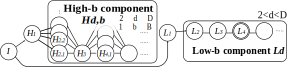
\includegraphics{img/model3.pdf}
 \caption{Example case exhibiting large bias in the branching factor depending on the subgraph.}
 \label{fig:model}
\end{figure}

Consider a blind search on the directed acyclic graph
shown in \refig{fig:model}.
The graph consists of two large components, \textbf{high-b} and \textbf{low-b} branches, and their entries $H_1,L_1$. The initial search node is $I$ and the goal node is $L_4$.
Both branches have maximum depth $D$, and the high-b branch has maximum width $B$.
Both $B$ and $D$ are very large.
This graph presents a pathological case for all of the previously described methods (\lifo, \fifo, \ro and type-based diversification), depending on successor ordering.
\lifo performs a DFS, and if \lifo first searches $H_1$ and the high-b branch due to successor ordering, it must explore the entire high-b branch before expanding $L_1$ and low-b branch.
\fifo performs Breadth-First Search (BreadthFS), and  will therefore suffer from the  high branching factor at depth 2 of the high-b branch, getting stuck before reaching $L_4$.
Although randomization can allow \ro to be better off than the behavior of \fifo/BreadthFS, the effect is limited:
For example, while expanding depth 2, \ro may occasionally expand depth 3 because it uniformly randomly selects a node from OPEN.
However, the probability of expanding nodes at depth 3 is initially only $1/(B+1)$ and continues to be small until  most of the nodes at depth 2 are expanded, 
because OPEN is mostly populated with the nodes from depth 2.
Depth-based diversification addresses the depth bias of BreadthFS.
However, even though it distributes the effort among various depths,
the probability of expanding $L_2,L_4$ at depths 2 and 4, is only $1/(B+1)$ each, which is very low when $B$ is very large.

We propose \;\emph{Invasion Percolation-based diversification (IP-diversification)}, a new diversification strategy for satisficing search that addresses this type of bias.
% in \refig{fig:model} for satisficing planning,%not limited to planning
% As discussed above, a diversification scheme seeks to allocate resources evenly among a group of nodes in order to avoid undesirable biases.
% One approach to implementing diversification is to treat diversification in a search graph as the problem of evenly covering the graph over time.
% By considering the graph as a multidimensional lattice, we can apply techniques that have been developed for modeling percolation in multidimensional lattices.
IP-diversification combines randomization and Prim's method \cite{prim1957shortest} for Minimum Spanning Tree (MST).
% -- we seek an unbiased method for evenly exploring a search graph based on this model.

\subsubsection{Invasion Percolation}

%which maps
%exactly into the Prim's method for minimal spanning tree problem \cite{prim1957shortest,barabasi1996invasion}.
%We first review Invasion Percolation, which  simulates the distribution of fluid
Invasion Percolation \cite{wilkinson1983invasion} simulates the distribution of fluid slowly %replacing/
invading porous media, e.g., water replacing the air in a porous rock.
We focus on a variant called bond IP (BIP), where ``bonds'' indicate edges in a lattice, and present the graph-based description by \citeauthor{barabasi1996invasion} (\citeyear{barabasi1996invasion}).
Given initial node(s) and a graph whose edges are assigned independent random values,
% Each node has a flag indicating whether Initial nodes are 
BIP iteratively marks the nodes.
Once assigned, the random value on each edge never changes.  The initial nodes are marked by default.
In each iteration marks an unmarked node to which the least-value outgoing edge leads.
Marked nodes represent the porous sites whose air is replaced by the water (invader).
% The algorithm proceeds as follows:
\citeauthor{barabasi1996invasion} (\citeyear{barabasi1996invasion}) showed that
this algorithm is equivalent to applying Prim's method for MST \cite{prim1957shortest} on a randomly weighted graph:
Prim's method constructs an MST by iteratively adding a neighboring edge with the least edge costs
to the existing tree.
% Since Prim's method works on any undirected graph, we can run BIP on arbitrary dimensions and graphs.
% Since Prim's method finds a MST minimizing the edge cost sum, BIP simulates the water greedily trying to expand with the least friction pathways.

% \begin{itemize}
%  \item Mark all initial nodes. 
%  \item In each iteration, select an edge with the least value among the edges which starts from marked nodes, then mark the destination of the edge.
% \end{itemize}

\begin{figure}[tb]
 \centering
 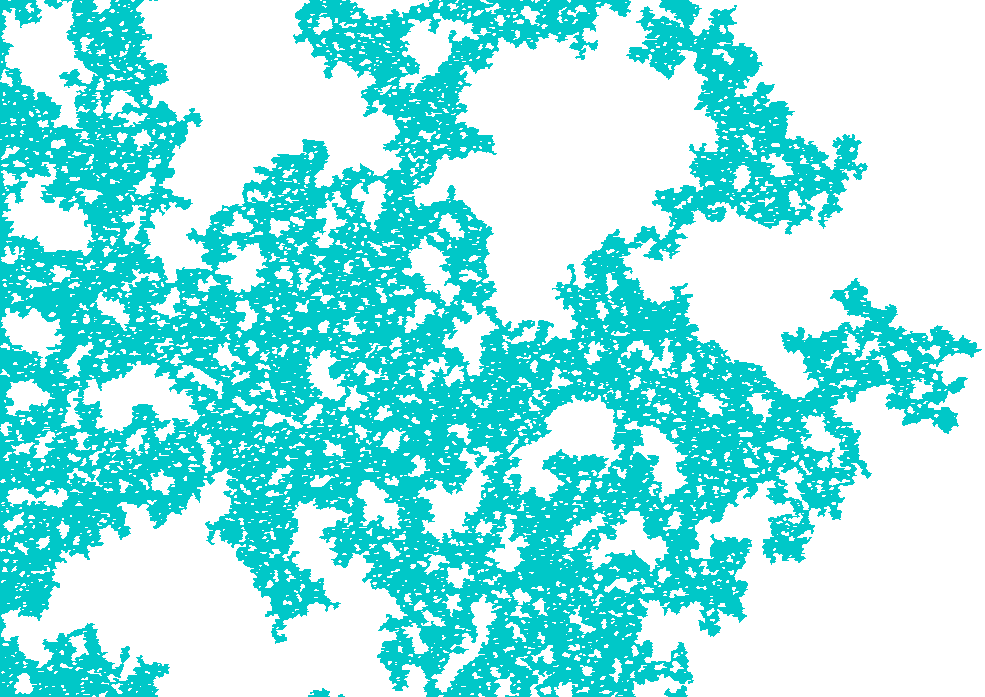
\includegraphics[width=0.4\linewidth]{img/static/ip.png}
 \caption{Invasion Percolation on 2-dimensional lattice}
 \label{fig:ip}
\end{figure}

\refig{fig:ip} illustrates a 2-D lattice after running BIP for a while. The initial nodes are 
at the leftmost edge of the rectangular region, i.e. the fluid percolates from the left. The
resulting structure has holes of various sizes that the fluid has not invaded, due to
the high-valued edges surrounding the neighbors of the holes, which serve as an embankment preventing the water from invading. Since the random value
on each edge is fixed, the algorithm does not mark the nodes inside the hole until it marks all nodes with smaller
random values in the entire space outside the embankments.
This behavior is critical to forming a fractal structure.

\subsubsection{Invasion Percolation for Search Diversification}
We adapt the BIP model as a exploration mechanism for best-first search.
%% doesnt look so important --- pretty obvious
% The basic idea is: Given a search graph that we would like to search in an unbiased manner,
% we treat it as a graph with randomly assigned edge costs and apply BIP.
Previous work on BIP was on physical simulations with relatively small graphs, 
and to our knowledge, this is the first application of BIP  to complex \emph{implicit} graphs.
% The original mapping from BIP to an equivalent graph algorithm (Prim's method) assumes an explicit representation of the graph. 
% Here, we adapt their method for the implicit graphs which are searched using BFS.


The actual implementation of BIP is quite simple:
%It can be implemented as
A % pseudo heuristic % in this case, just calling $\bip$ a ``function'' seems sufficient -- no need to invent new term
function $\bip$ returns a randomly selected value 
for each search edge that caused the node to be evaluated.
%It is important to note that this random value must be memoized, i.e.,
For each edge, the function should always return the same value  once a random value is assigned to that edge. This requires storage whose size is linear in the number of edges that are explored.
% While it is possible to avoid this storage with a random hash function such as Zobrist hash \cite{zobrist1970new}, the preliminary experiment showed that it incurs the additional cost of node evaluation. Therefore, we simply generate a new value by a pseudo random number generator.

% While a naive implementation assigns a random value to  an operator / search node pair, this results in much larger memory
% usage and also incurs more search overhead per node (e.g., instantiating a pair, increased cost of retrieving the
% memoized value from the cache). Thus, in our implementation, we assign a random integer value to a search
% node and to an operator separately, then take the XOR of the values.

For intra-plateau exploration, $\bip$ is used to break ties in a plateau induced by the primary heuristic function $h$, i.e. $[h,\bip,*]$.
Since nodes are sorted in increasing order of the memoized random value attached to each edge, the node expansion order within a plateau follows that of Prim's method.
For inter-plateau exploration, we alternate the expansion between standard GBFS and a queue sorted by $\bip$: $\mit{alt}([h],[\bip])$, just as in Type-GBFS.


%moving this after the ``IP for diversification'' heading because this text mentions search and expansions
Consider applying BIP to the DAG in \refig{fig:model}.
There is a non-negligible probability that the search finds the solution without expanding high-b branch:
This occurs when the value $v(H_1)$ of $H_1$ is higher than the value of any of $L_1\ldots L_4$,
whose probability is 1/5
 (follows from $\int_0^1 dv(H_1) Pr(\forall i; v(L_i)\leq v(H_1)) = \int_0^1 x^4dx$). 
In this case, node $H_1$ is acting as an embankment, causing nodes in the  low-b branch to be expanded.
In contrast, the opposite case is very unlikely:
$L_1$ \emph{could} be expanded after expanding all of $H_{d,b}$ for $1\leq d\leq 4$ and $1\leq b \leq B$,
 but the probability of this,  $1/(2B+3)$,  is very small (assuming large $B$).

Also consider the case when $H_1$ is expanded with probability $4/5$.
Even if this embankment is broken, $H_3$ could act as another embankment again with probability $1/5$.
Moreover, it also avoids expanding large number of nodes in $H_{2,i}$ whose values are higher than $L_1\ldots L_4$.
$B/5$ of the nodes are not expanded on average because each node is not expanded with the same probability $1/5$.

Thus, at every possible ``bottleneck'' in the search space that forms an embankment, BIP tends to start looking at the other branches.
Since this is affected by the least width of a subgraph rather than the maximum,
it is less likely to suffer from the pathological behavior exemplified by \refig{fig:model}.

% This shape is known as a random fractal whose Hausdorff dimension is less than the space dimension.

Node expansion order according to $\bip$ differs  significantly from that of \ro (pure random selection).
% 
\ro is equivalent to performing a random sort and select the first node, i.e., \ro essentially assigns a \emph{new} random value to \emph{all} nodes at every single expansion.
In contrast, $\bip$ assigns a value to each edge only once, which develops embankments and allows unexplored ``holes'' to have longer lifetimes.
% 
% In $\bip$, once a hole is surrounded by high-valued edges, it keeps being unexplored until all low-valued edges are traversed. This embankment prevents exploration into the hole and is critical to forming a fractal structure.
% 
Consider what would happen if we switch the behavior from $\bip$ to \ro starting from the state shown in \refig{fig:ip}. Since all nodes are assigned a new random value at each expansion, the embankment nodes are more likely to be expanded, filling the holes more quickly. Thus, running \ro results in a more solid, denser expansion biased to the left, near the initial nodes.





There is one difference between the assumptions made by BIP/Prim \cite{barabasi1996invasion} and classical planning.
The search spaces of classical planning are directed while BIP/Prim assumes undirected graphs. Thus, although Prim's method finds the minimum spanning tree on an undirected graph, it may not return the minimum-weight tree on a directed graph. This, however, does not affect the completeness of our search algorithm because it just changes the order of expansion (BIP-based search diversification does not prune any nodes).
% 
% If used as intra-plateau diversification,
% The expected quality of the solution does not change, up to tiebreaking. In order to find better solutions with GBFS, one can sort the nodes preferring smaller $g$ value for tiebreaking, i.e. $[h,g,*]$ sorting strategy, but it does not preclude us from applying $\bip$ for further tiebreaking, i.e. $[h,g,\bip,*]$. Although these are possible, in this paper we solely focus on satisficing solutions for the sake of clarity and simplicity. Evaluating the impact of such $g$-based tiebreaking scheme on the solution cost is an avenue of future work.
% 
% Finally, 
Adopting algorithms for minimum spanning arborescence for directed graphs \cite{chu1965shortest,edmonds1967optimum,tarjan1977finding,gabow1986efficient} to search diversification is a direction for future work.%. However, currently we have  no straightforward way to adopt these algorithms for diversification. (A direction for future work.)


\subsubsection{Search Behavior of IP-diversification}

We analyze the basic search behavior of IP-diversification by applying a blind search on IPC satisficing instances.
We ran four configurations, namely Type-based diversification with depth $d$ (hd:$[\depth]$) and IP-diversification (hb:$[\bip]$), as well as BreadthFS (h:$[\fifo]$) and random search (ro:$[\ro]$).
All solvers were given a 3 min/4GB resource limit.

We plotted the depth of the nodes expanded by these algorithms on two representative runs (\pddl{visitall-sat11-p20, tidybot-sat11-p08}) in \refig{fig:distribution}.
As expected, \ro behaves similarly to BreadthFS/\fifo (search is biased to the shallow depths) and
Depth-diversification shows a flat distribution because it is specifically designed to achieve the fair allocation among depths.
% avoid using ``effective branching factor'' without enough discussion
Compared to BreadthFS/\fifo and \ro, the increase of nodes-per-depth by IP-diversification is much slower, supporting our observation that IP is controlled by the least width in the search graph.
Compared to Type-based diversification which shows linear nodes-per-depth, IP still exhibits exponential behavior because IP has no explicit mechanism for balancing  the search  efforts wrto depths. However, IP expands smaller number of nodes in the shallower region.
Similar figures were obtained for other domains.

\begin{figure}
 % \includegraphics{img/ipc2011-sat/barman-sat11/p20-intra.pdf}
 %% because barman is ``flat'' in a sense it does not have peaks but also ``bumpy'' in a sense that it has lots of noise
 \includegraphics{img/ipc2011-sat/visitall-sat11/p20-intra.pdf}
 %% it is more reasonable to use the successful domain in the next table 
 \includegraphics{img/ipc2011-sat/tidybot-sat11/p08-intra-mod.pdf}
 % \includegraphics{img/ipc2011-sat/elevators-sat11/p16-intra.pdf}
 \caption{Distribution of the evaluated nodes per depth.}
 \label{fig:distribution}
\end{figure}

We also compared their performance on IPC instances.
% in order to assess their pure effects not affected by any particular heuristics.
% We compared the performance of 
% (h) Standard GBFS,
% (hd) depth-based diversification $[h,\depth]$ and
% (hb) IP diversification $[h,\bip]$.
% Due to the characteristics of Blind heuristics which always returns a constant value 1, the only meaningful diversification is intra-plateau diversification.
\reftbl{tbl:blind} shows that both (hd) and (hb) improves upon blind BreadthFS while 
not strictly dominating each other: (hb) shows better performance than
(hd) on the \pddl{Tidybot} domain.
Comparison between \ro and hb indicate that the blind performance of IP is better than that of \ro in \pddl{tidybot} and \pddl{pegsol}.
% Thus, the base performance of (hd), (hb) and (ro) are shown to 
% These indicate that IP is a good candidate for improving the performance of heuristic search.

\begin{table}[bt]
\centering
\relsize{-1}
% \setlength{\tabcolsep}{0.4em}
\begin{tabular}{l|rrr|r}
   & h         & hb             & hd                & \ro       \\
 % & $[\fifo]$ & $[\bip,\fifo]$ & $[\depth,\fifo]$  & $[\ro]$ \\
\hline
ipc2014 sum  & 14 & 15        & \bi{22}   & 15\\
\hline
% cavediving & 7  & 7         & 7         & 7\\
hiking       & 2  & 2         & \bi{7}    & 2\\
tetris       & 0  & 1         & \bi{3}    & 1\\
% thoughtful & 5  & 5         & 5         & 5\\
\hline
ipc2011 sum  & 30 & 48        & \bi{50.8} & 35\\
\hline
% nomystery  & 3  & 4         & 4         & 4\\
pegsol       & 17 & 18.5      & \bi{19}   & 17\\
scanalyzer   & 4  & 4         & \bi{6}    & 4\\
sokoban      & 3  & 3         & \bi{3.8}  & 3\\
tidybot      & 2  & \bi{17.5} & 14        & 6\\
visitall     & 0  & 0         & \bi{3}    & 0\\
\hline
\end{tabular}
\caption{Problems solved with 3 minutes/4GB RAM (average of 10 runs).
% (hd) and (hb) are not dominating each other and (hb) and (\ro) are different.
Best results are in \textbf{bold}.
We do not show the domains with no differences between configurations.
}
\label{tbl:blind}
\end{table}

\subsection{Evaluation of IP-Diversification} 

% in order to minimize the effect of domain configuration problem
% \cite{vallati2015effective} (e.g. successor ordering caused by the way actions are described in PDDL).

% \subsubsection{Evaluation under Eager GBFS}

Given the performance of blind search,
IP-diversification is a good candidate for improving the performance of diversified heuristic search.
% In this section, we evaluate the effects of type-based diversification and IP-diversification on Eager GBFS, where nodes are evaluated as soon as they are generated.
% Since the effect of diversification could be heuristic-dependent, we tested $\ff$ and $\cg$.
% Following the previous work \cite{valenzano2014comparison,xie14type}, all configurations are evaluated under unit cost transformation
%  because we are solely focused on the coverage and the first solution.
% This is natural because GBFS has no guarantee on the plan cost.
% Also, according to \cite[p6, left, middle]{xie14type}, Type-GBFS does not incur significant loss in solution quality.
% 
% Finally, since depth diversification works only within plateaus, it does not change the best-first order wrto $h$
% value and it is unlikely to have significant change in solution quality except for some noise from the randomness
% in tiebreaking.
% 
%% not included --- its is a pseudo heuristics anyways
% , Landmark-Count (LC) heuristics\cite{richter2008landmarks}
% 
We compared the performance of 
(h), the standard GBFS, with
the combined Type-based diversification (hdD) from \refsec{sec:gbfs-comparison}
as well as intra-plateau  IP-diversification (hb:$[h,\bip]$), inter-plateau IP-diversification (hB:$alt([h],[\bip])$), and combined intra/inter-plateau IP diversification (hbB:$alt([h,\bip],[\bip])$).
% All configurations uses \fifo default tie-breaking which is the default configuration in Fast Downward,
% except Type-bucket in Type-GBFS (which uses \ro, as specified in their paper).
%(\textbf{See \reftbl{tbl:lazy-supplemental} in supplements for Lazy-GBFS results, where heuristic value of parents are used.})
% (\textbf{See Supplemental \reftbl{tbl:eager-supplemental} for comparisons to the other default tie-breaking methods (\lifo and \ro). \reftbl{tbl:lazy-supplemental} also contains Lazy-GBFS results, where heuristic value of parents are used}.)
\todo*{\ro GBFS evaluation}

\begin{table}[htbp] 
\setlength{\tabcolsep}{0.2em}
\centering
\begin{tabular}{|ll|r|rrr|r|r|rrr|r|}
% \begin{tabularx}{\linewidth}{|ll|l|l|lll|l|l|lll|}
\hline
& & \multicolumn{ 5}{c|}{$\cg$} & \multicolumn{ 5}{c|}{$\ff$} \\ 
   &       & h   & {hb}           & {hB}           & {hbB}                & {hdD}                & h   & {hb}           & {hB}           & {hbB}          & {hdD}         \\ 
   &       &     & {intra}        & {inter}        & {both}               & {both}               &     & {intra}        & {inter}        & {both}         & {both}        \\ \hline
%  &total  & 228 & 232.5          & 261.8          & \textbf{268.5}       & 263.2                & 231 & 261.5          & 297.7          & \textbf{307.4} & 280.6         \\ \hline \multirow{14}{0.4em}{\rotatebox{90}{\textbf{\relsize{-1}IPC2011}}}
   &total  & 187 & 187.2          & 206.8          & \textit{208.7}       & \textbf{215.8}       & 192 & 207.8          & 232.9          & \textbf{237.7} & 223.9         \\ \hline \multirow{8}{1em}{\rotatebox{90}{\textbf{\relsize{-1}IPC11 w/o duplicates}}}
%  &barman & 0   & 0              & 0              & 0                    & 0                    & 8   & 8.1            & \bred{16.2}    & \bred{15.2}    &         10.3  \\ 
   &elevators & 9   & 9.2            & \bred{12.6}    & \bred{13.3}          & \textbf{9.7}         & 19  & 18.2           & 18.5           & 19.4           & 13.7          \\ 
 % &floortile & 0   & 0              & \bred{0.6}     & \bred{0.5}           & \textbf{2}           & 6   & 4.6            & 5.6            & 5.2            & \textbf{6.9}  \\ 
   &nomystery & 7   & 6.4            & 5.5            & 5.6                  & \textbf{15.1}        & 9   & 6.6            & 7.6            & 6.6            & \textbf{17}   \\ 
 % &openstacks & 10  & \borange{12}   & \borange{13.5} & \borange{13.6}       & 12.8                 & 11  & \borange{19.2} & \borange{17.7} & \borange{19}   & 15.8          \\ 
   &parcprinter & 20  & 19.6           & 13.7           & 12.4                 & 18.7                 & 20  & 20             & 19.9           & 18.9           & 20            \\ 
 % &parking & 18  & \borange{19.2} & \borange{19.4} & \borange{19.9}       & 14.1                 & 11  & \borange{16.8} & \borange{13.3} & \borange{16.9} & \textbf{17.2} \\ 
   &pegsol & 20  & 20             & 19.7           & 19.8                 & 20                   & 20  & 20             & 20             & 20             & 20            \\ 
   &scanayzer & 20  & 20             & 20             & 20                   & 20                   & 15  & 16.6           & \bred{19.1}    & \bred{19.1}    & \textbf{18.6} \\ 
   &sokoban & 16  & 15.9           & 15.8           & 15.2                 & \textbf{17}          & 19  & 18.6           & 18.5           & 18.4           & 17.4          \\ 
   &tidybot & 16  & \borange{17.3} & \borange{17.5} & \borange{17.5}       & \textbf{18.6}        & 16  & 15             & 16.4           & {16.3}         & \textbf{16.7} \\ 
 % &transport & 10  & 10.2           & \bred{11.5}    & \bred{15.6}          & \textbf{12.1}        & 0   & 0              & {0.2}          & \textbf{1.3}   & 0.2           \\ 
 % &visitall & 3   & 3.9            & \bred{10}      & \bred{10.2}          &         6.4          & 3   & \borange{5}    & \borange{11.8} & \borange{12.1} & 6.3           \\ 
   &woodworking & 2   & 1.8            & \bred{14}      & \bred{12.8}          &         \textbf{7.7} & 2   & 1.5            & \bred{14.8}    & \bred{15.7}    & \textbf{7.2}           \\ \hline \multirow{14}{1em}{\rotatebox{90}{\textbf{\relsize{-1}IPC14}}}
   &barman & 0   & 0              & 0              & 0                    & 0                    & 0   & 0              & \bred{7.6}     & \bred{6.5}     & \textbf{1}             \\ 
   &cavediving & 7   & 7.1            & 7              & 6.9                  & 7                    & 7   & 7              & 7              & 7              & 7.2           \\ 
   &childsnack & 1   & 0              & 0.1            & 0                    & \textbf{1.5}         & 0   & 0              & 0.1            & 0              & 0.3           \\ 
   &citycar & 0   & {0.2}          & \textbf{1.1}   & {0.4}                & \textbf{4.7}         & 0   & 0              & \bred{3}       & \bred{3.8}     & \textbf{7.1}  \\ 
   &floortile & 0   & 0              & \bred{0.5}     & \textcolor{red}{0.2} & \textbf{2}           & 2   & 2              & 2.1            & 2              & 2.1           \\ 
   &ged    & 0   & 0              & \bred{4.8}     & \bred{4.6}           & \textbf{9.7}         & 19  & 19.2           & 12.8           & 13             & 13.8          \\ 
   &hiking & 18  & 15.9           & \bred{18.7}    & \bred{18.8}          & \textbf{19.7}        & 20  & 17.6           & 19.9           & 20             & 20            \\ 
   &maintainance & 16  & 14.6           & 14.9           & 14.1                 & 15.8                 & 11  & 6.7            & 10             & 5.8            & 11.1          \\ 
   &openstacks & 0   & 0.1            & \bred{2.5}     & \bred{2.4}           &         \textbf{0.5} & 0   & \borange{15.7} & \borange{11.7} & \borange{14.5} & \textbf{7}             \\ 
   &parking & 7   & \bblue{10.4}   & 7.6            & \bblue{10.9}         & 4.1                  & 4   & \bblue{5.4}    & 2.3            & \bblue{4.8}    & \textbf{5.7}  \\ 
   &tetris & 18  & \bblue{19.7}   & 17.6           & \bblue{19.4}         & 14.3                 & 1   & \borange{8.6}  & \borange{7}    & \borange{11.1} & \textbf{4.9}           \\ 
   &thoughtful & 5   & 4.9            & 5.2            & 5.2                  & 5                    & 8   & \borange{9.1}  & \borange{11.2} & \borange{11}   & \textbf{13.1} \\ 
   &transport & 5   & 4.1            & \bred{6}       & \bred{7.1}           & 4.7                  & 0   & 0              & 0              & 0              & 0             \\ 
   &visitall & 0   & 0              & \bred{2}       & \bred{2.1}           & 0                    & 0   & 0              & \bred{3.4}     & \bred{3.8}     & 0             \\ 
\hline
% \end{tabularx}
\end{tabular}
\caption{
Number of solved instances (5 min, 4Gb RAM), mean of 10 runs.
\textbf{h}: baseline GBFS.
\textbf{hb/hB}: intra / inter-plateau IP diversification $[h,\bip]$ and $alt([h],[\bip])$,
\textbf{hbB}: A combined IP configuration $alt([h,\bip],[\bip])$,
\textbf{hdD}: $alt([h,\brackets{d}],[\brackets{g,h},\ro])$ (same as hdD from \reftbl{tbl:results})  . % confusing because hdD is not IP-based
The same highlighting/coloring rules as \reftbl{tbl:results} are applied, showing that
% Results follow the same observation made in \reftbl{tbl:results}.  
intra/inter-plateau schemes based on IP are complementary.
\textbf{bold} shows the improvements by \textbf{hdD}.
Although \textbf{hbB} and \textbf{hdD} are comparable overall,
per-domain comparison shows \textbf{hbB} and \textbf{hdD} are complementary.
}
\label{tbl:results2}
\end{table}


% In order to remove the effect of randomness of the algorithm, we
% implemented a deterministic version of Type-based queue for Type-GBFS
% which, instead of selecting a bucket at random, iterates over the
% buckets in a reverse order that each bucket is introduced.
% Similarly, the diversification based on the depth is not randomized but
% is implemented as a loop-based implementation.

Results are shown in \reftbl{tbl:results2}. IP-diversification, applied to both
intra- and inter-plateau exploration, resulted in improvements on both the $\ff$ and $\cg$ heuristics.
Complementary effects similar to \reftbl{tbl:results} are observed between hb and hB, and  hbB outperforms both hb and hB.
This provides additional empirical evidence for the hypothesis that intra/inter-plateau exploration  are complementary, and that they can be combined to yield superior performance.

Overall, hbB performs comparably to hdD. However, note that some domains were improved by Type-based but not by IP (e.g. \pddl{nomystery, sokoban, childsnack})
or vise versa (\pddl{transport, visitall}).
% 
% For example, with $\cg$, (hb) outperforms (hd) on \pddl{parking14} and \pddl{tetris14}, while
% \pddl{openstacks14} and \pddl{childsnack14} are solved only by (hd) and other configurations have 0 coverage.
% Similarly with $\ff$, while (hb) improves performance on \pddl{visitall11} ($3.0\rightarrow 5.3$), (hd) does not, and
%  and vice versa on \pddl{childsnack14} ($0.0\rightarrow 4.0$ by (hd)).
% 
These results indicate that Type-based and IP diversification are orthogonal,
addressing different diversity criteria (depth vs breadth).

\section{Intra- and Inter-Plateau Diversification on a State-of-the-Art Planner} % \sota kind of risky, but this time, I think we justfified usage of \sota  better by relating it to Jasper and Probe
% separating this out to once again remind readers of the intra-inter contribution

Up to this point, we have evaluated intra/inter-plateau exploration on greedy best-first search in order to cleanly isolate their effect.
Next, we evaluate the combined effect of intra/inter-plateau exploration when applied to a state-of-the-art planner,
% (\textbf{See Supplemental \reftbl{tbl:lama-supplemental} for configurations not listed in \reftbl{tbl:results}.})
% 
the LAMA2011 configuration in the current version of FastDownward,
which incorporates a number of search enhancement techniques such as lazy evaluation, multi-heuristic search and preferred operators.
In order to focus on coverage, we only run the first iteration (unit-cost GBFS) of LAMA, 
denoted as $alt([\ff],\pref{\ff},[\lc],\pref{\lc})$, where
% $\ff$ denotes the FF heuristics,
$\lc$ denotes the landmark-count heuristic
and $\pref{X}$ denotes the preferred operator queue with sorting strategy $X$.


% As additional baselines, we also include coverages for Probe \cite{LipovetzkyG11} and Jasper \cite{xie14ipc}, which are \sota, non-portfolio planners from the IPC'14 agile track, 
% Jasper combines Type-LAMA with GBFS-LS \cite{XieH14gbfsle}, which starts a local GBFS when 
% the number of expansion in the current local minima exceeds a certain threshold.
% %While this method address the problem of large plateau, it does not address the diversity
% %within plateau.
% %Also, since Jasper is based on an older LAMA, %
% We also include the original LAMA'11 implementation.
% %In our environment, Probe and Jasper did not outperform the original LAMA'11.
% %This is presumably due to the difference in the CPU speed (AMD@2.36GHz in IPC14 vs our Intel Haswell@2.9GHz), resulting in more search being performed in 5 minutes on our machines vs. the machines used in the IPC14 agile track competition.
% The latest FastDownward LAMA configuration performs better significantly better than the other baselines.


% Since our version is based on the latest FastDownward, we also tested the original version used in IPC2011.
% 
% Type-LAMA \cite{xie14type} 
% adds Type-based buckets $\brackets{g,h}$ to the list of alternating queues in LAMA, and is denoted as: 
% $alt\left([\ff],\ldots,\pref{\lc},\brackets{g,\ff}\right)$.

% We followed the best configuration suggested by \citeauthor{xie14type} (\citeyear{xie14type})
% for Type-GBFS, which uses the type vector $\brackets{g,\ff}$.

We apply the methods proposed in this paper incrementally.
We first add a single exploration strategy to LAMA.
(d, b) augments $[h]$ with type-based and IP diversification for intra-plateau exploration ($[h,\depth]$ and $[h,\bip]$), respectively.
(D, B) incorporates inter-plateau exploration by adding $\brackets{g,\ff}$ and $[\bip]$ to LAMA's alternation queue, respectively.
LAMA+D is equivalent to Type-LAMA \cite{xie14type}.
Next, we combine intra/inter-plateau diversification methods:
(dD) applies both changes in (d) and (D), and similarly (bB) applies both changes in (b) and (B).

Finally, (db$^2$DB) incorporates all 4 methods into LAMA.
Let $db$ denote $alt(\depth,\bip)$, alternation between depth and IP based diversification for intra-plateau exploration,
and let $DB$ denote $alt(\brackets{g,\ff},\bip)$, alternation between type-based and IP based diversification for inter-plateau exploration.
The resulting configuration,
LAMA-db$^2$DB, incorporates all of the ideas proposed in this paper: {\small $alt\big([\ff,db], \pref{\ff}, [\lc,db], \pref{\lc}, DB\big)$.}
This configuration alternates between type-based and IP diversification in each iteration.
It allocates 1/5 of the entire search time to inter-plateau exploration 
(same as the frequency with which Type-LAMA selects from $\brackets{g,\ff}$),
so it spends 1/10 of the time on $[\bip]$ and 1/10 of the time on $\brackets{g,\ff})$.
Adopting more sophisticated approaches for determining exploration frequency \cite{schulte2014balancing,nakhost2009monte} is a direction for future work.
%\citeauthor{schulte2014balancing} (\citeyear{schulte2014balancing}) combined Tree-search framework
%\cite{keller2013trial} with UCT \cite{kocsis2006bandit} to automatically adjust the ratio of exploration %in Classical Planning.
%Similarly, Arvand \cite{nakhost2009monte} uses Random Walk Local Search for exploration,
%with sophisticated mechanism for balancing the ratio. %Since our LAMA-Btdb uses a trivial approach for determining the exploration ratio (fixed to 1/5),
%Adopting these exploration-ration tuning approaches is a direction for future work.

% supplement?
%Since this experimental setting (satisficing, 5min limit) is similar to the Agile track of the IPC, 
% we also include results for Probe \cite{LipovetzkyG11}, which had the highest coverage in the 2014 IPC Agile track, as another baseline.


%% removed ``once every 5 expansions to be the same as TGBFS'' both because it was unclear what it meant, and also, it wasn't clear why it's desirable to match the Type-GBFS exploration rate.
%in order to explore at the same rate as Type-GBFS, we
%(once for every 5 expansions).

% \begin{center}
\begin{tabular}{lr}
 & coverage\\
\hline
Probe & 319\\
LAMA & 386.2\\
Type-LAMA & 387.3\\
LAMA-bB & \\
LAMA-dD & \\
LAMA-dbBD & 397.5\\
LAMA-bdbdBD & 398.3\\
\end{tabular}
\end{center}

\begin{table*}[htbp]
\setlength{\tabcolsep}{0.4em}
\centering
\begin{tabular}{ll|llllllll}
% \begin{tabularx}{\linewidth}{ll|ccc|llllllll}
\hline
 &            & \multicolumn{8}{c}{Planners Based on the Latest FastDownward} \\
 % 
 &            & LAMA   & +{d}           & +{D}             & +{dD}            & +{b}           & +{B}             & +{bB}          & +{db$^2$DB}      \\ 
 &total       &{293.2} & {296.5}        & {294.3}          & {295.4}          & {293.3}        & {287.6}          & {297.6}        & {\textbf{304.5}} \\ \hline \multirow{8}{1em}{\rotatebox{90}{\textbf{IPC11 w/o duplicates}}}
 &elevators   &20      & 19.3           & 19               & 19.2             & 20             & 19.4             & 19.9           & 19.6             \\ 
 &nomystery   &10      & 9.9            & \bred{17.4}      & \bred{16.4}      & 9.8            & 10.4             & 9.7            & \bred{16.1}      \\ 
 &parcprinter &20      & 18.4           & 19.9             & 19.7             & 18.2           & 19.5             & 18.3           & 19.3             \\ 
 &pegsol      &20      & 19             & 20               & 20               & 19.4           & 20               & 20             & 20               \\ 
 &scanalyzer  &19      & 19.3           & 19.1             & 19.2             & \borange{19.5} & \borange{19.6}   & \borange{19.5} & 19.2             \\ 
 &sokoban     &17      & 16.9           & 16.9             & 16.6             & 16.4           & 17               & 16.9           & 16.2             \\ 
 &tidybot     &16      & \textbf{17}    & 15.8             & 15.8             & 14.8           & 15.7             & \textbf{16.5}  & \textbf{16.5}    \\ 
 &woodwork    &20      & 20             & 20               & 20               & 20             & 20               & 20             & 20               \\ \hline \multirow{14}{1em}{\rotatebox{90}{\textbf{IPC14}}}
 &barman      &15      & 13.6           & 9.5              & 10.4             & 12.1           & \textbf{16}      & 14.2           & 14               \\ 
 &cavediving  &7       & 7              & 7.1              & 7.1              & 6.8            & 6.9              & 6.7            & 7                \\ 
 &childsnack  &0       & \textbf{9.3}   & 0.1              & 0                & 0.2            & 0.3              & 0.1            & 0                \\ 
 &citycar     &2       & 1              & \borange{5.5}    & \borange{4.4}    & \borange{4.5}  & \borange{4.2}    & \borange{4.1}  & \borange{4.4}    \\ 
 &floortile   &2       & 2              & 2.1              & 2                & 2              & 2                & 2              & 2                \\ 
 &ged         &20      & 20             & 20               & 20               & 20             & 20               & 20             & 20               \\ 
 &hiking      &18.5    & 18.7           & 17.5             & 18.7             &  \bblue{19.1}  & 17.5             &  \bblue{19.6}  & 18.8             \\ 
 &maintenance &1       & 1              &   \bred{5.5}     &   \bred{5.6}     & 1              & 1                & 1              &   \bred{3.6}     \\ 
 &openstacks  &20      & 20             & 20               & 20               & 20             & 20               & 20             & 20               \\ 
 &parking     &19.1    & \textbf{19.8}  & 16.7             & 18.7             & \textbf{19.6}  & 18.1             & 18.7           & \textbf{19.6}    \\ 
 &tetris      &9.3     & 7.1            & 7.4              & 7.1              &  \bblue{12.4}  & 4.7              &  \bblue{15.3}  &  \bblue{14.2}    \\ 
 &thoughtful  &14      & \borange{14.5} &   \borange{15.1} &   \borange{15.4} & 13.1           &   \borange{14.5} & 12.9           &   \borange{14.6} \\ 
 &transport   &3.3     &  \bblue{3.8}   & 2.6              &  \bblue{3.8}     &  \bblue{4.4}   & 3.7              &  \bblue{3.8}   & 3.5              \\ 
 &visitall    &20      & 18.9           & 17.1             & 15.3             & 20             & 17.1             & 18.4           & 15.9             \\ \hline
\end{tabular}
\caption{
Number of solved instances in 5min,4GB RAM.
 % is based on a newer version of FastDownward and its
LAMA's sorting strategy is $alt([\ff],\pref{\ff},[\lc],\pref{\lc})$.
For each heuristic $h=\ff$ and $h=\lc$ in LAMA,
 % +d, +D, +dD, +b, +B, +bB adds the exploration:
(d,b) augments $[h]$ with type-based and IP diversification for intra-plateau exploration ($[h,\depth]$ and $[h,\bip]$, respectively).
%(D=Type-LAMA \cite{xie14type}, B) uses respective diversification for inter-plateau exploration by adding $\brackets{g,\ff}$ and $[\bip]$ to LAMA's alternation queue.
(D,B) applies inter-plateau exploration by adding $\brackets{g,\ff}$ and $[\bip]$ to LAMA's alternation queue, respectively. D corresponds to Type-LAMA \cite{xie14type}.
(dD) includes both changes in (d) and (D) (similarly for (bB), (b) and (B)).
Finally, (db$^2$DB) combines all methods:
{\small $alt\big([\ff,alt(\depth,\bip)], \pref{\ff}, [\lc,alt(\depth,\bip)], \pref{\lc}, alt(\brackets{g,\ff},\bip)\big)$.}
The same highlighting rules as \reftbl{tbl:results} are applied.
LAMA+db$^2$DB combines improvements from 4 diversification strategies and achieved the best overall coverage.
% In the right columns, Jasper'14, Probe'14, LAMA'11 are the original versions used in IPC'14/'11.
}
\label{tbl:lama}
\end{table*}
% & Jasper'14 & Probe'14 & LAMA'11 
% & 248       & 241      & 271     
% & 20        & 16       & 19      
% & 4         & 6        & 11      
% & 6         & 14       & 20      
% & 20        & 20       & 19      
% & 16        & 17       & 20      
% & 16        & 13       & 16      
% & 18        & 17       & 16      
% & 19        & 20       & 20      
% & 20        & 20       & 20      
% & 6         & 1        & 7       
% & 0         & 0        & 0       
% & 5         & 9        & 1       
% & 0         & 2        & 2       
% & 18        & 19       & 20      
% & 19        & 20       & 6       
% & 12        & 14       & 6       
% & 18        & 0        & 20      
% & 0         & 6        & 4       
% & 6         & 1        & 7       
% & 15        & 16       & 16      
% & 0         & 6        & 8       
% & 10        & 4        & 13      

\reftbl{tbl:lama} shows the number of solved instances.
Each single diversification improved the overall performance of LAMA except LAMA+B.
For combinations of two methods (dD and bB),
complementary effects by intra-/inter-plateau diversification similar to \reftbl{tbl:results} are observed.
Although LAMA+B did not result in improvement, adding B to LAMA+b resulted in larger coverage in LAMA+bB.
Finally, bd$^2$BD outperformed all other methods.
We observed complementary effects from dD and bB, each addressing different diversity criteria.
% Type-based exploration sometimes significantly degrades LAMA performance when the heuristic is correct but ignored in favor of the type-based queue. 

%\section{Related Work} % let's remove the Related Work section because right now, the contents are 100% IP-related, and makes it look as though IP should be viewed as the most important contribution.

% Valenzano14 baseline discussion moved to IP section.

% too dangerous because there's no clear example of a "continuous space" which is clearly better suited for IP than novelty. replaced below in conclusions+future work with a more positive type of mention.
% % "novelty metric" itself needs to be mentioned, although we cant cite BWFS ...
% While novelty metric used in Probe \cite{LipovetzkyG11} or IW \cite{lipovetzky2012width} also addresses diversity of a new node from existing nodes, one drawback is that it assumes a propositional representation of the problem. As such, currently there is no straightforward way to compute the novelty metric on domains where no such representation is available. In contrast, IP-diversification only assumes the graph-based representation of the explored problem space and therefore, for example, the same method can be applied to the sampled nodes in a continuous space without modification, given the background theories on Percolation Physics on continuous space.
% The analysis in this direction is future work.

% removed 30 years
%  (\emph{real world is continuous})

% \section{Related Work}
% 
% Other techniques that can be viewed as addressing breadth-biases are
% symmetry breaking \cite{Fox1998,pochter2011exploiting,domshlak2013symmetry}
% and partial order reduction \cite{hall2013faster,wehrle2013relative}.
% While these are usually described as ``pruning techniques'',
% they can be viewed as diversification techniques, in that 
% \emph{they aim to remove the bias for a set of redundant nodes.}
% % 
% Suppose we have a set of nodes $S=\{a_1, a_2, b, c\}$ where the subset
% $A=\{a_1, a_2\}$ is ``redundant'' according to some measure (e.g. by symmetry, partial order). 
% A search algorithm which selects a node randomly from $S$ for expansion is clearly biased -- 
% group $A$ is twice as likely to be expanded than either $b$ or $c$, although $a_1$ and $a_2$ are ``same'' nodes.
% By eliminating either $a_1$ or $a_2$, symmetry and partial-order reduction eliminates this bias.


% Seems safer to remove this, because Lelis et al 2013 is applied to sliding tiles, blocksworld, pancake, so claiming their work is for trees doesn't look right.
%% The previous work on Type system \cite{lelis2013stratified} has also used the number of children with particular
%% heuristic value. Although this could be another direction to address the breadth-related bias, our work is
%% significantly different --- First, we focus on the search on a general graph rather than a tree. Second, they claim
%% ``type system can use any information about a node to define its type'', without further explanation why this
%% metric works.



\section{Conclusions and Future Work}

In this paper, we first introduced the notion of \emph{Intra}- and
\emph{Inter}-plateau exploration in satisficing heuristic search.
While  previous work on exploration focused on inter-plateau exploration,
we argued that intra-plateau exploration addresses orthogonal issues, and showed that 
the type-based diversification framework originally developed for inter-plateau diversification could be used to unify intra- and inter-plateau diversification.
We then showed empirically that these two modes of diversification have 
orthogonal, complementary effects when implemented as diversification strategies for GBFS, % although "complementary" implies that they can be combined, this is worth explicitly emphasizing
and showed that it is possible to combine intra/inter-plateau diversification, 
resulting in better performance than either class of strategy alone.

Next, we showed that type-based diversification is not sufficient for bias avoidance in graphs where nodes have largely varying number of neighbors, and proposed IP-diversification, a new breadth-aware diversification strategy which addresses this issue. We then showed that IP-diversification can be used as either intra- or inter-plateau exploration strategy, i.e., IP is a dual-mode diversification strategy unlike depth-diversification and $\brackets{g,h}$ type-based diversification, which are specialized for either intra- or inter-plateau exploration. %"bimodal" can be misinterpreted in the probability distribution sense of two peaks.
In addition, to our knowledge, this is the first successful fractal-inspired planning algorithm.

Finally, we showed that incorporating these two new ideas (performing both intra/inter-plateau exploration, and IP-diversification) into FD/LAMA yields state-of-the-art performance on IPC benchmark instances. 

While this paper investigated Bond-IP (the variant of Invasion Percolation which fixes random values to edges),
the dual variant which fixes values on nodes is called \emph{Site IP}.
Analysis of SIP is a direction for future work as they could have different fractal characteristics \cite{sheppard1999invasion}.
%Fractal analysis on the search graph is an interesting avenue of future work.
\citeauthor{valenzano2014comparison} (\citeyear[Section 4.3]{valenzano2014comparison}) evaluated a baseline, knowledge-free heuristic which assigns a random $h$-value to a node.
By itself, this would behave similarly to the $ro$ baseline strategy, if heuristic values are reevaluated for reopened nodes (the default behavior in FastDownward\footnote{\relsize{-1}\url{http://hg.fast-downward.org/file/df227b467100/src/search/search_engines/eager_search.cc\#l202}}).
However, \citeauthor{valenzano2014comparison} disabled node-reopening in all their experimental configurations, which, in effect, fixes the random value for each node and makes them behave similarly to SIP.

% XXX I think this paragraph was in the submission to avoid questions about comparisons vs novelty, but no longer necessary in the final version.
%This paper has shown that various knowledge-free strategies can be plugged in as inter/intra-plateau exploration.
%In future work, we seek to employ more blind search methods such as novelty-based metrics \cite{lipovetzky2012width} in this two-tiered exploration architecture.
%A general, principled framework for quantifying search biases, perhaps incorporating notions such as partial order and symmetry \cite{pochter2011exploiting,domshlak2013symmetry,hall2013faster,wehrle2013relative}, is a direction for future work.
% {\bf [Added this paragraph because a conclusion section which only repeats our contributions seemed too empty without adding some broad discussion / direction for future work -- but now it's over the page limit -- some of the above symm/po refs should be pruned.]}

While we focused on ``pure'' satisficing search w/o quality consideration, we note that the IPC Quality score of GBFS with $\ff$ and diversification has improved by 25\% from the baseline because of the increased coverage (not shown due to space). Yet, pure satisficing search is beneficial in its own right as a tiebreaking strategy in \astar \cite{Asai2017}. In future work, we will evaluate the effectiveness of the proposed methods in that context.


